%%%%%%%%%%%%%%%%%%%%%%%%%%%%%%%%%%%%%%%%%%%%%%%%%%%%%%%%%%%%%%%%%%%%%%%%%%%%%%%%
%2345678901234567890123456789012345678901234567890123456789012345678901234567890
%        1         2         3         4         5         6         7         8

\documentclass[letterpaper, 10 pt, conference]{ieeeconf}  % Comment this line out
                                                          % if you need a4paper
%\documentclass[a4paper, 10pt, conference]{ieeeconf}      % Use this line for a4
                                                          % paper

\IEEEoverridecommandlockouts                              % This command is only
                                                          % needed if you want to
                                                          % use the \thanks command
\overrideIEEEmargins
% See the \addtolength command later in the file to balance the column lengths
% on the last page of the document



% The following packages can be found on http:\\www.ctan.org
\usepackage{graphicx} % for.png, bitmapped graphics files
%\usepackage{epsfig} % for postscript graphics files
%\usepackage{mathptmx} % assumes new font selection scheme installed
%\usepackage{times} % assumes new font selection scheme installed
%\usepackage{amsmath} % assumes amsmath package installed
%\usepackage{amssymb}  % assumes amsmath package installed
\usepackage{float}
\usepackage[section]{placeins}

\usepackage{xcolor} % Required for specifying custom colours

\colorlet{mdtRed}{red!50!black}

\usepackage[colorlinks=true, urlcolor=mdtRed, citecolor=mdtRed, linkcolor=mdtRed,border={0 0 0}]{hyperref}
\usepackage[backend=biber,style=numeric,autocite=superscript,sorting=none]{biblatex} 
\usepackage{setspace}

\addbibresource{bio.bib} 

\onecolumn
\title{\LARGE \bf
Applications of Mass Spectrometry in Molecular Diagnostics
}

%\author{ \parbox{3 in}{\centering Huibert Kwakernaak*
%         \thanks{*Use the $\backslash$thanks command to put information here}\\
%         Faculty of Electrical Engineering, Mathematics and Computer Science\\
%         University of Twente\\
%         7500 AE Enschede, The Netherlands\\
%         {\tt\small h.kwakernaak@autsubmit.com}}
%         \hspace*{ 0.5 in}
%         \parbox{3 in}{ \centering Pradeep Misra**
%         \thanks{**The footnote marks may be inserted manually}\\
%        Department of Electrical Engineering \\
%         Wright State University\\
%         Dayton, OH 45435, USA\\
%         {\tt\small pmisra@cs.wright.edu}}
%}

\author{Christopher Eeles, Minoru Nakano, Michael Lau, Abubakar Mohamed % <-this % stops a space
}

\begin{document}

\maketitle
\thispagestyle{empty}
\pagestyle{empty}

\setstretch{1.6}
% Table of Contents
%%%%%%%%%%%%%%%%%%%%%%%%%%%%%%%%%%%%%%%%%%%%%%%%%%%%%%%%%%%%%%%%%%%%%%%%%%%%%%%%
\setcounter{secnumdepth}{3}
\setcounter{tocdepth}{3}
\tableofcontents % Prints the main table of contents

\setstretch{1}

\twocolumn
%%%%%%%%%%%%%%%%%%%%%%%%%%%%%%%%%%%%%%%%%%%%%%%%%%%%%%%%%%%%%%%%%%%%%%%%%%%%%%%%

% Abstract
%%%%%%%%%%%%%%%%%%%%%%%%%%%%%%%%%%%%%%%%%%%%%%%%%%%%%%%%%%%%%%%%%%%%%%%%%%%%%%%%
\begin{abstract}

This non-exhaustive review is intended to introduce the reader to Mass Spectrometry (MS) and its application to the rapidly growing field of molecular diagnostics. In this review we will focus on applications of MALDI and ESI to the field of molecular diagnostics.

\end{abstract}
%%%%%%%%%%%%%%%%%%%%%%%%%%%%%%%%%%%%%%%%%%%%%%%%%%%%%%%%%%%%%%%%%%%%%%%%%%%%%%%%

% Introduction to Mass Spectrometry
%%%%%%%%%%%%%%%%%%%%%%%%%%%%%%%%%%%%%%%%%%%%%%%%%%%%%%%%%%%%%%%%%%%%%%%%%%%%%%%%
%%%%%%%%%%%%%%%%%%%%%%%%%%%%%%%%%%%%%%%%%%%%%%%%%%%%%%%%%%%%%%%%%%%%%%%%%%%%%%%%
\section{\textbf{Introduction to Mass Spectrometry}}
%%%%%%%%%%%%%%%%%%%%%%%%%%%%%%%%%%%%%%%%%%%%%%%%%%%%%%%%%%%%%%%%%%%%%%%%%%%%%%%%
%%%%%%%%%%%%%%%%%%%%%%%%%%%%%%%%%%%%%%%%%%%%%%%%%%%%%%%%%%%%%%%%%%%%%%%%%%%%%%%%

    % What is MS?
    \textbf{What is MS?}\hfill
    \vspace{5 pt}

    Mass spectrometry is a method and set of instrumentation for sorting and detecting atoms or molecules on the basis of mass to charge ratio (m/z)\autocite{R7}. MS has been used extensively in chemistry from as early as the 1940s, later being adapted for biological and organic chemistry.\autocite{R7} However, applications for complex biological molecules---such as nucleic acids, glycopeptides, etc---were prevented due fragmentation caused by the high energy bombardment needed to vaporise samples. This problem was overcome with the discovery of "soft ionization" techniques with lower energy vaporisation in the late 1980s. Since then MS has become increasingly specialized for use in the biological and medical sciences.\autocite{R7} 

    \vspace{5 pt}

    % Fig 1
    \begin{figure}[h]
        \centering
    
        \fbox{
            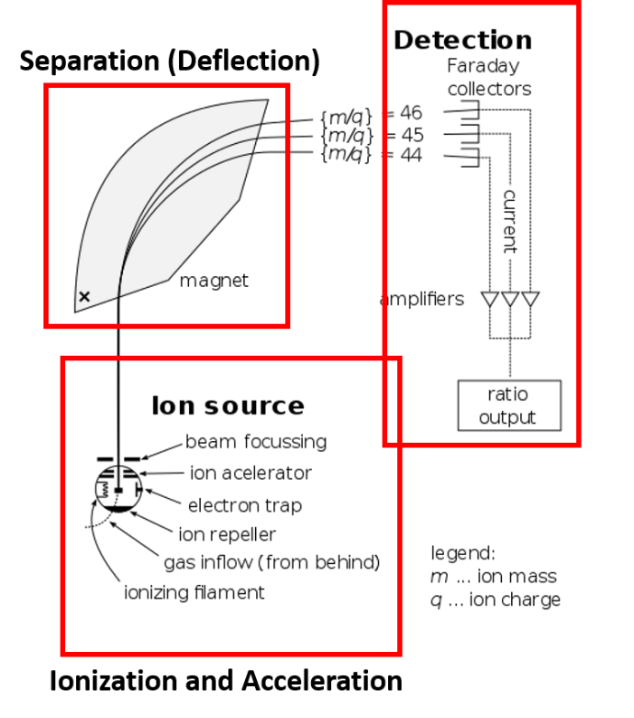
\includegraphics[width=3in]{Figures/Fig23.png}
        }
        \caption{Schematic of a Simple Mass Spectrometer\autocite{R9}}

    \end{figure}

    % Why is MS Relevant to Molecular Diagnostics
    \textbf{Why is MS Relevant to Molecular Diagnostics?}\hfill
    \vspace{5 pt}

    Accuracy, high-throughput and multiplexing are becoming essential characteristics for all biomedical instrumentation.\autocite{R7} As such MS is emerging as a powerful tool in proteomics, genomics, metabolomics and other fields of basic research. Moreover, advances in these fields generate myriad new targets and pathways for medical intervention, diagnostic or otherwise. As information about biological processes continues to increase mass spectrometry will have a significant role to play in both basic and applied research.

    \FloatBarrier

    % MS Technical Background 
    %%%%%%%%%%%%%%%%%%%%%%%%%%%%%%%%%%%%%%%%%%%%%%%%%%%%%%%%%%%%%%%%%%%%%%%%%%%%%%%%
    \subsection[\textbf{MS Technical Background}]{\textbf{MS Technical Background}\autocite{R7}}

        % Fig 2
        \begin{figure}[h]
            \centering
        
            \fbox{
                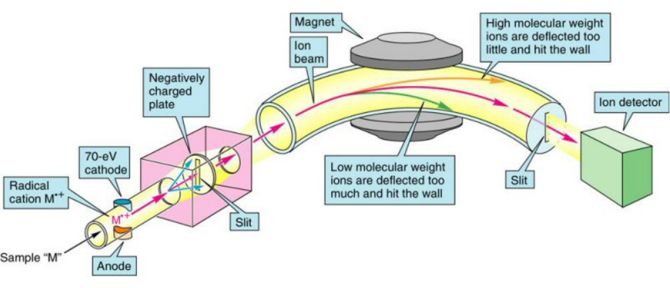
\includegraphics[width=3in]{Figures/Fig5.png}
            }
            \caption{Deflection Mass Spectrometer\autocite{R7,R9}}
        \end{figure}

        Mass Spectrometry is a method for sorting and detecting atoms or molecules based on the ratio of their mass to charge. The system outputs the mass to charge ratio (m/z) for each detected particle, which is plotted against the intensity of each detection. The goal of mass spectrometry is to subject a sample, usually of unknown chemical composition, to five steps which will ultimately separate atoms by mass and charge. The sample is placed within a vacuum to isolate other particulates and gases, so the analysis will only run on the sample. The stages of mass spectrometry are outlined as follows:

        % Fig 3
        \begin{figure}[h]
            \centering
        
            \fbox{
                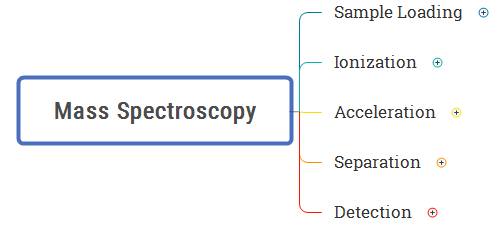
\includegraphics[width=3in]{Figures/Fig1.png}
            }
            \caption{Process of Mass Spectrometry}
        \end{figure}

        % Sample Loading        
        %%%%%%%%%%%%%%%%%%%%%%%%%%%%%%%%%%%%%%%%%%%%%%%%%%%%%%%%%%%%%%%%%%%%%%%%%%%%%%%%
        \subsubsection{\textbf{Sample Loading}}\hfill\hfill
        \vspace{5 pt}

            % High Performace Liquid Chromatography (HPLC)
            \textbf{High Performance Liquid Chromatography (HPLC)}\hfill

            A method for physically separating components of a mixture by interaction of immiscible stationary and mobile phases. 

            % Fig 4
            \begin{figure}[h]
                \centering
            
                \fbox{
                    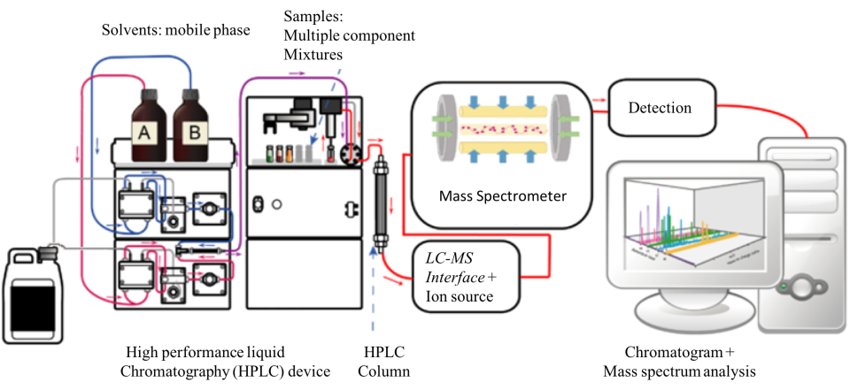
\includegraphics[width=3in]{Figures/Fig8.png}
                    
                }
                \caption{HPLC System\autocite{R9}}
            \end{figure}


            % Automated Array Loading
            \textbf{Automated Array Loading} \hfill

            Use micro-arrays, a mechanical arm, and a HPLC tube to yield automated, high-throughput, multiplexed sample analysis.

            % Fig 5
            \begin{figure}[h]
                \centering
            
                \fbox{
                    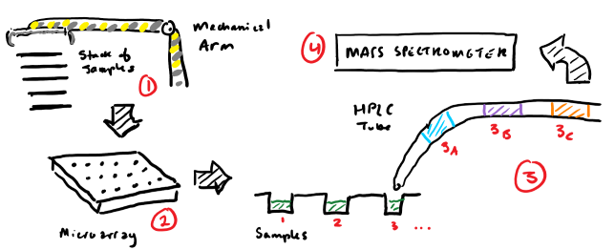
\includegraphics[width=3in]{Figures/Fig9.png}
                }
                \caption{Automated Array Loader}
            \end{figure}

            \FloatBarrier

        % Ionization
        %%%%%%%%%%%%%%%%%%%%%%%%%%%%%%%%%%%%%%%%%%%%%%%%%%%%%%%%%%%%%%%%%%%%%%%%%%%%%%%%
        \subsubsection{\textbf{Ionization}}\hfill \hfill

         % Fig 6
         \begin{figure}[h]
            \centering
            
            \fbox{
                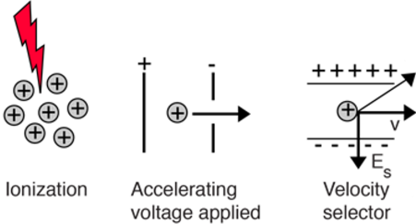
\includegraphics[width=3in]{Figures/Fig11.png}
            }
            \fbox{
                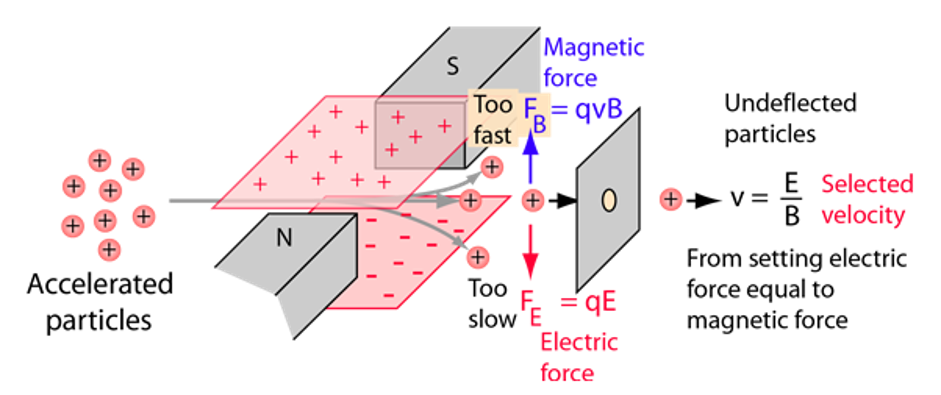
\includegraphics[width=3in]{Figures/Fig12.png}
            }

            \caption{Ionization (Top) and Mass Selector (Bottom)}
            \tiny{\url{http://hyperphysics.phy-astr.gsu.edu/hbase/magnetic/maspec.html}}

        \end{figure}

        Traditional MS uses high-energy EM or particle beams to knock electrons off the sample. These high energy beams tend to fragment or destroy organic molecules, historically preventing biological applications of MS. Both solid and liquid samples can be ionized in this way. The result is a positively charged gas which passes into the vacuum of the acceleration chamber due to negative pressure.
        \FloatBarrier  

        % Acceleration
        %%%%%%%%%%%%%%%%%%%%%%%%%%%%%%%%%%%%%%%%%%%%%%%%%%%%%%%%%%%%%%%%%%%%%%%%%%%%%%%%
        \subsubsection{\textbf{Acceleration}}\hfill
            
            % Fig 7
            \begin{figure}[h]
                \centering
                \fbox{
                    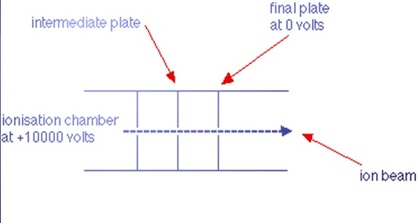
\includegraphics[width=3in]{Figures/Fig26.png}
                }  
                \caption{Acceleration Chamber}
                \tiny{\url{http://chemicalinstrumentation.weebly.com/mass-spectrometry.html}}
            \end{figure}

        The acceleration chamber is a vacuum thus vaporized sample ions enter the chamber due to negative pressure. A voltage is applied across two metal plates, accelerating the ions to the desired kinetic energy. A mass selector deflects ions of the wrong kinetic energy, allowing a stream of ions with identical KE to pass through a slit into the separator. Therefore, when the ions reach the mass analyzer the only properties differentiating them are their mass and charge.

        % Separation
        %%%%%%%%%%%%%%%%%%%%%%%%%%%%%%%%%%%%%%%%%%%%%%%%%%%%%%%%%%%%%%%%%%%%%%%%%%%%%%%%        
        \subsubsection{\textbf{Separation}}\hfill

        The method used to isolate the ions for detection based on mass/charge ratio (m/z). Traditionally used deflection but modern MS technology have alternatives depending on the requirement of the experiment.
        
            \textbf{Magnetic Deflection\autocite{R7}}\hfill

            \begin{figure}[h]
                \centering

                \fbox{
                    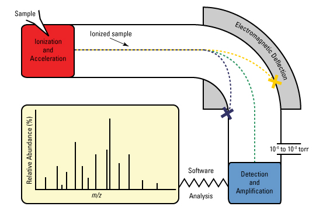
\includegraphics[width=3in]{Figures/Fig13.png}
                }
                \caption{A Deflection Based Mass Analyzer}
                \tiny{\url{https://en.wikipedia.org/wiki/Time-of-flight_mass_spectrometry}}

            \end{figure}

            The ions pass through a magnetic field and are deflected with electromagnetic forces. Different types of ions can be identified and detected, since ions with different masses would have different deflection behaviors. Sample ions enter with equal kinetic energy. Ions with smaller masses or higher charges are deflected more. The detector outputs plots the m/z value for all detected particles.

            \FloatBarrier

            \textbf{Time of Flight (TOF)} \hfill

            Ionized compounds with different mass and charge travel at speeds. Compounds can therefore be be identified by measuring the time they take to travel a known distance. Sample ions enter with equal kinetic energy. Therefore velocity is proportional to charge and inversely proportional to mass. First particles detected are lightest, increasing proportional to time.

            \begin{figure}[H]
                \centering
            
                \fbox{
                    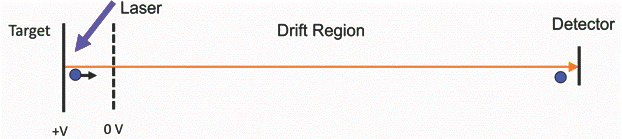
\includegraphics[width=3in]{Figures/Fig14.png}
                }
                \caption{A Time of Flight Based Mass Analyzer}

                \tiny{\url{https://en.wikipedia.org/wiki/Time-of-flight_mass_spectrometry}}

            \end{figure}

            \FloatBarrier
        
        % Detection
        %%%%%%%%%%%%%%%%%%%%%%%%%%%%%%%%%%%%%%%%%%%%%%%%%%%%%%%%%%%%%%%%%%%%%%%%%%%%%%%%
        \subsubsection[\textbf{Detection}]{\textbf{Detection}\autocite{R9}} \hfill \hfill
        \vspace{5 pt}

        Records either the charge induced, current produced, or photons generated when ions pass by or collide with a surface. First generation mass spectrometers used photo-plates to make images of the detected samples. Modern systems detect voltage changes at a given location and send these to a computer to output a m/z plot. Typically, an electron multiplier is used, but Faraday cups and ion-to-photon detectors are also used depending on the MS design specifications.

        \vspace{5 pt}
            
            \textbf{Location Based}

            \begin{figure}[h]
                \centering
            
                \fbox{
                    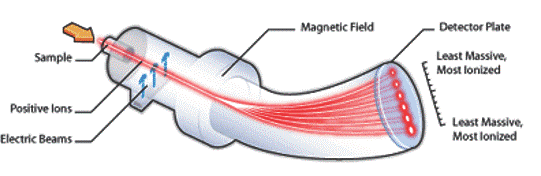
\includegraphics[width=3in]{Figures/Fig15.png}
                }
                \caption{Location Based MS Detector}

                \tiny{\url{https://www.scq.ubc.ca/mass-spectrometry/​}}

            \end{figure}

            Deflected ions hit the surface of an amplifier. The positions hit by these ions are detected, and graphed according to intensity and location. Using this information, quantity and mass of each ion in the sample can be determined, and the mass of the sample molecule can be calculated.

            \textbf{Time Based}

            \begin{figure}[h]
                \centering
            
                \fbox{
                    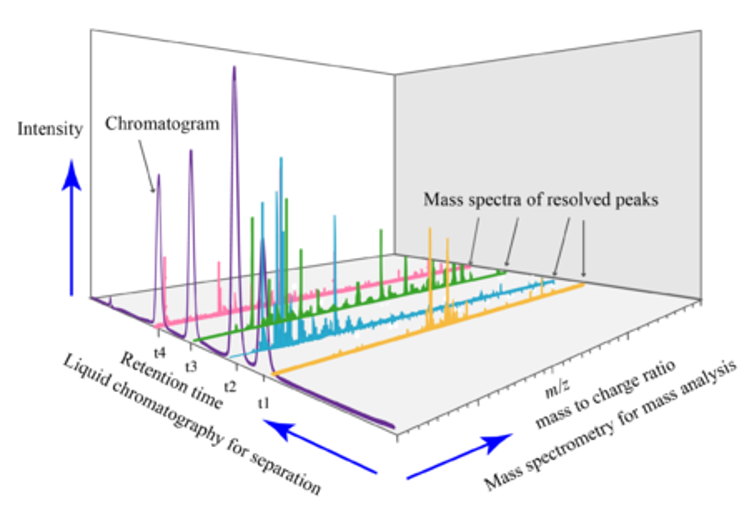
\includegraphics[width=3in]{Figures/Fig16.png}
                }
                \caption{Time Based MS Detector Output}

                \tiny{\url{https://en.wikipedia.org/wiki/Liquid_chromatography%E2%80%93mass_spectrometry​}}

            \end{figure}

            A detector measures voltage changes in a plate to high time resolution. This system can be multiplexed by time spacing incoming samples via liquid chromatography. The output of a multiplexed time of flight mass spectrometer is displayed in Fig 11.

            \FloatBarrier
    %%%%%%%%%%%%%%%%%%%%%%%%%%%%%%%%%%%%%%%%%%%%%%%%%%%%%%%%%%%%%%%%%%%%%%%%%%%%%%%%
    \subsection{\textbf{A Brief History of Mass Spectrometry}}
    %%%%%%%%%%%%%%%%%%%%%%%%%%%%%%%%%%%%%%%%%%%%%%%%%%%%%%%%%%%%%%%%%%%%%%%%%%%%%%%%
        \begin{figure}[h]
            \centering
        
            \fbox{
                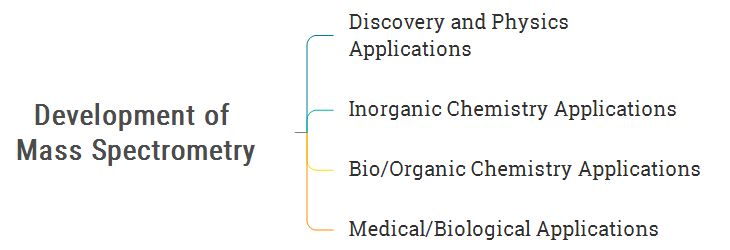
\includegraphics[width=3in]{Figures/Fig3.png}
            }
            \caption{History of MS Development}
        \end{figure}

        % Discovery and Applications
        %%%%%%%%%%%%%%%%%%%%%%%%%%%%%%%%%%%%%%%%%%%%%%%%%%%%%%%%%%%%%%%%%%%%%%%%%%%%%%%%
        \subsubsection[\textbf{Discovery and Physics Applications}]{\textbf{Discovery and Physics Applications}\autocite{R8}}\hfill \hfill

        The physics necessary for MS was developed in the 1890s by Cambridge Professor J.J. Thomson. His work on cathode rays (electron beams) rewarded him with a Nobel Prize in 1906 for using EM deflection to estimate the mass of the electron. By the 1940s the technique was commonly used in physics laboratories, but were constructed by engineers on site and therefore inaccessible to other fields of study.

        \vspace{5 pt}

        % Inorganic Chemistry Applications
        %%%%%%%%%%%%%%%%%%%%%%%%%%%%%%%%%%%%%%%%%%%%%%%%%%%%%%%%%%%%%%%%%%%%%%%%%%%%%%%%
        \subsubsection[\textbf{Inorganic Chemistry Applications}]{\textbf{Inorganic Chemistry Applications}\autocite{R8}}\hfill \hfill

        Electrical Engineer Alfred Nier commercialized and promoted MS use outside of the physics community. As a result, by the 1950s it became widely adopted in the field of industrial chemistry---mostly for quantifying the amount of each component in a mixture.

        \vspace{5 pt}

        % Bio/Organics Chemistry Applications
        %%%%%%%%%%%%%%%%%%%%%%%%%%%%%%%%%%%%%%%%%%%%%%%%%%%%%%%%%%%%%%%%%%%%%%%%%%%%%%%%
        \subsubsection[\textbf{Bio/Organic Chemistry Applications}]{\textbf{Bio/Organic Chemistry Applications}\autocite{R8}}\hfill \hfill 
        
        The work of American Chemist Fred McLafferty, Klaus Biemann, and Carl Djerassi characterized the mass spectra of known compounds. These spectra were arranged into a library of mass signatures which was used to identify unknown compounds in mixtures by matching them to known spectra. Eventually the technique advanced enough to predict the complex structures of organic compounds. By the 1980s small organic molecules were regularly being analyzed with MS.

        \vspace{5 pt}

        % Medical/Biological Applications
        %%%%%%%%%%%%%%%%%%%%%%%%%%%%%%%%%%%%%%%%%%%%%%%%%%%%%%%%%%%%%%%%%%%%%%%%%%%%%%%%
        \subsubsection[\textbf{Medical/Biological Applications}]{\textbf{Medical/Biological Applications}\autocite{R8}}\hfill \hfill

        In 1988, novel "soft ionization" techniques---MALDI and ESI---were developed. These tools allow for ionization of large molecules without an excess amount of energy being deposited into the compounds. John Fenn received the Nobel Prize in Chemistry in 2002 for the development of ESI. During his acceptance speech he famously stated that his technique provided “electrospray wings for molecular elephants”. These techniques and their application in molecular diagnostics will be discussed in detail presently.

    %%%%%%%%%%%%%%%%%%%%%%%%%%%%%%%%%%%%%%%%%%%%%%%%%%%%%%%%%%%%%%%%%%%%%%%%%%%%%%%%
    %%%%%%%%%%%%%%%%%%%%%%%%%%%%%%%%%%%%%%%%%%%%%%%%%%%%%%%%%%%%%%%%%%%%%%%%%%%%%%%%
    \section{\textbf{Biological Mass Spectrometry}}
    %%%%%%%%%%%%%%%%%%%%%%%%%%%%%%%%%%%%%%%%%%%%%%%%%%%%%%%%%%%%%%%%%%%%%%%%%%%%%%%%
    %%%%%%%%%%%%%%%%%%%%%%%%%%%%%%%%%%%%%%%%%%%%%%%%%%%%%%%%%%%%%%%%%%%%%%%%%%%%%%%%

    Mass spectrometry has high accuracy, sensitivity and wide dynamic range that can be utilized in high-throughput capacities. This has allowed MS to have countless applications in life sciences.\autocite{R1} Currently, MS has been successfully used for molecular diagnostics of microbial and viral infections.\autocite{R7} Furthermore, new developments expand the application to public health evaluations and clinical fields. In this section we will be discussing ESI and MALDI MS methods as applied to molecular diagnostics.

    A recently discovered cancer biomarkers were identified using tissue cultures, taking advantage of mass spectrometry-based proteomics instrumentation during experimentation. Discovery of such biomarkers is essential for accurate diagnosis and monitoring of cancer patients, and is becoming crucial for treatment and prevention. Almost all proteomic bio-marker discovery platforms use mass spectrometry\autocite{R10}. In this case, they used ESI-MS, and concluded that the capability of MS demonstrates significant potential as a tool for the discovery and validation of candidate biomarkers.\autocite{R10}

        %%%%%%%%%%%%%%%%%%%%%%%%%%%%%%%%%%%%%%%%%%%%%%%%%%%%%%%%%%%%%%%%%%%%%%%%%%%%%%%%
        \subsection{\textbf{Matrix Assisted Laser Desorption Ionization}}
        %%%%%%%%%%%%%%%%%%%%%%%%%%%%%%%%%%%%%%%%%%%%%%%%%%%%%%%%%%%%%%%%%%%%%%%%%%%%%%%%
        An ionization technique that uses a laser energy absorbing matrix to create ions from large molecules with minimal fragmentation.\autocite{R5} Ionization of the matrix allows samples to "piggy-back" into the vapour without absorbing too much of the applied energy. Thus the unstable bonds in complex biological molecules are retained, allowing analysis of compounds previously too fragile for study via MS.\autocite{R5}

        \begin{figure}[h]
            \centering
        
            \fbox{
                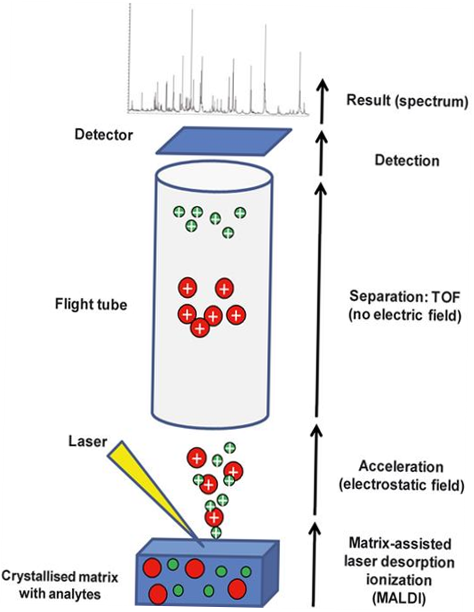
\includegraphics[width=3in]{Figures/Fig19.png}
            }
            \caption{Schematic of a MALDI-MS System}

            \tiny{\url{http://www.wikiwand.com/en/Matrix-assisted_laser_desorption/ionization#/Time_of_Flight}}

        \end{figure}

            \subsubsection[\textbf{Matrix Assisted Laser Desorption}]{\textbf{Matrix Assisted Laser Desorption Ionization (MALDI)}} \hfill \hfill
        
            An ionization technique that uses a laser and an energy absorbing matrix to create ions from large molecules with minimal fragmentation. Samples are prepared by embedding them within pre-matrix material. The resulting mixture crystallizes sample within matrix, influenced heavily by presence of small acidic molecules. A laser is used to irradiate the sample, triggering the release of fragment molecules from the mixture. The analyte molecules are ionized in an electromagnetic field and accelerated into the mass analyzer such that kinetic energies are all equal.\autocite{R1}

            \begin{figure}[h]
                \centering
            
                \fbox{
                    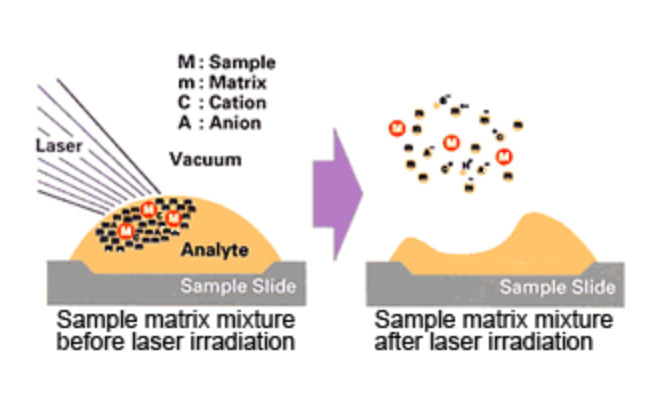
\includegraphics[width=3in]{Figures/Fig4.png}
                }
                \caption{Diagram of Ionizing Matrix}

                \tiny{\url{https://en.wikipedia.org/wiki/Necrotizing_enterocolitis}}

            \end{figure}

            % Matrix Composition 
            %%%%%%%%%%%%%%%%%%%%%%%%%%%%%%%%%%%%%%%%%%%%%%%%%%%%%%%%%%%%%%%%%%%%%%%%%%%%%%%%
            \subsubsection[\textbf{Matrix Composition}]{\textbf{Matrix Composition}\autocite{R1,R5}} \hfill \hfill

            The defining feature of this technique is the use of a solid or semi-solid matrix to analyze samples. Such matrices vary in composition and are specifically tailored for the biomolecule to be analyzed as well as type of laser to be used. This allows for a comprehensive array of potential analytes to be tested, from intact microorganisms to large protein molecules.

            Example matrices used most frequently include:
            \begin{itemize}
                \item{2,5-dihydroxbenzoic acid (DHB)}
                \item{α-cyano-4-hydroxycinnamic acid (CHCA)}
                \item{Sinapinic acid (SA)}
                \item{Ferulic acid (FA)}
            \end{itemize}
            Considerations when choosing the matrix molecule:
            \begin{enumerate}
                \item{Size: Low molecular weight to allow easy vaporization but large enough not to evaporate during sample preparation.}
                \item{Acidity: Acidic molecules act as a source of proton to encourage ionization   of the analyte.}
                \item{Absorption Range: High optical absorption range in either the UV or IR range  to efficiently absorb laser irradiation. This can be achieved by molecules     with conjugated double bonds.}
                \item{Presence of polar groups: Molecules with polar groups is functional aqueous solutions.}
            \end{enumerate}
            The mixture of the organic solvent and water allows both hydrophobic and hydrophilic molecules to dissolve into the solution. CHCA, FA, SA show to be more effective for detection of proteins, while DHB is suited to detection of glycopeptides.

        % MALDI Applications in Molecular Diagnostics
        %%%%%%%%%%%%%%%%%%%%%%%%%%%%%%%%%%%%%%%%%%%%%%%%%%%%%%%%%%%%%%%%%%%%%%%%%%%%%%%%
        \subsection{\textbf{MALDI Applications in Molecular Diagnostics}}

            \subsubsection[\textbf{Nectrotizing Enterocolitits}]{\textbf{Necrotizing Enterocolitis}\autocite{R2}}\hfill \hfill

            NEC is a devastating disease that affects the bowels of premature infants. MALDI/TOF is used to quickly analyze fecal samples and find differences between the mutant and the functional protein responsible for the condition. It can be used as a means of pre-symptomatic diagnosis helping health care providers to prevent progression of this devastating inflammatory bowel disease in premature infants. In the lab, fecal samples are cultured and isolated then identified using MALDI-TOF; bio-markers identified with this technique assist in the development of screening tools to allow for early diagnosis and treatment. The uniqueness strengths of MALDI-TOF allow for the fecal samples that would have been unavailable in traditional mass spectrometry due to the delicate nature of the bio-marker molecules.

            \begin{figure}[h]
                \centering
            
                \fbox{
                    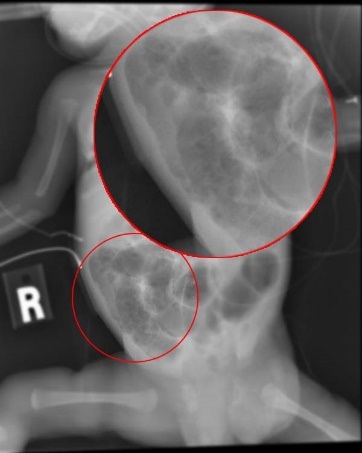
\includegraphics[width=3in]{Figures/Fig24.png}
                }
                \caption{X-ray of Baby with Necrotizing Eneterocolitis}
                \tiny{\url{https://en.wikipedia.org/wiki/Necrotizing_enterocolitis}}

            \end{figure}

            % Pancreatic Cancer
            %%%%%%%%%%%%%%%%%%%%%%%%%%%%%%%%%%%%%%%%%%%%%%%%%%%%%%%%%%%%%%%%%%%%%%%%%%%%%%%%
            \subsubsection[\textbf{Pancreatic Cancer}]{\textbf{Pancreatic Cancer}\autocite{R3,R4,R10}}\hfill \hfill

            Membrane proteins have been identified as potential targets for anticancer drugs as well as bio-markers for early diagnosis. Recent studies have used MALDI-TOF mass spectrometry to isolate, analyze and identify membrane proteins unique to pancreatic cancer cells. This allowed them to identify a number of proteins associated with various cellular processes regulated by pancreatic cancer cells. These findings demonstrate the potential of MALDI MS for identifying large protein molecules from samples thereby helping to diagnose conditions and diseases through recognizable bio-markers.

            \begin{figure}[h]
                \centering
            
                \fbox{
                    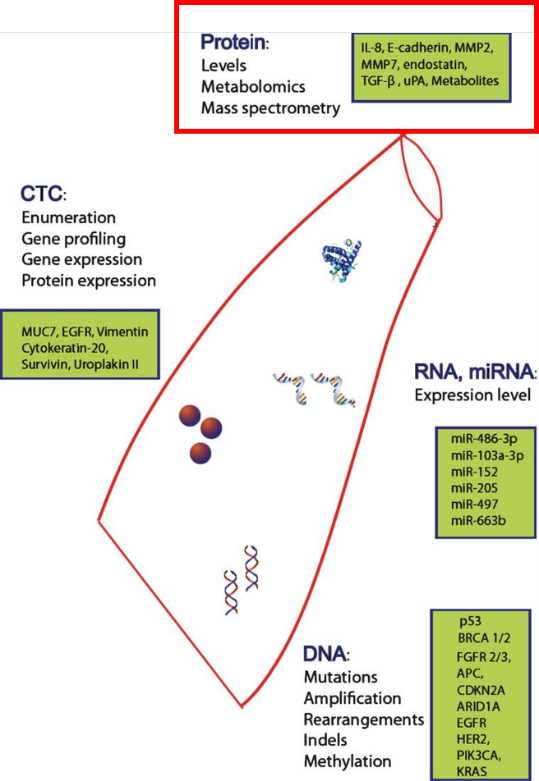
\includegraphics[width=3in]{Figures/Fig25.png}
                }
                \caption{Diagram of Biomarkers for Bladder Cancer}

                \tiny{\url{https://content.iospress.com/articles/bladder-cancer/blc160075}}

            \end{figure}


            % Identifying Drug Resistance in Bacteria
            %%%%%%%%%%%%%%%%%%%%%%%%%%%%%%%%%%%%%%%%%%%%%%%%%%%%%%%%%%%%%%%%%%%%%%%%%%%%%%%%
            \subsubsection[\textbf{Identifying Drug Resistance in Bacteria}]{\textbf{Identifying Drug Resistance in Bacteria}\autocite{R12}}\hfill \hfill

            MALDI/TOF serves as a method for determining the drug resistance of bacteria, especially to β-lactams (Penicillin family). It detects the presence of carbapenemases, which indicates drug resistance to standard antibiotics. In non-resistant bacteria, you would not expect to find such compounds as they facilitate cell death.

        % Electron Ionization Mass Spectrometry (ESI-LS)   
        %%%%%%%%%%%%%%%%%%%%%%%%%%%%%%%%%%%%%%%%%%%%%%%%%%%%%%%%%%%%%%%%%%%%%%%%%%%%%%%%
        \subsection[\textbf{Electrospray Ionization Mass Spectrometry}]{\textbf{Electrospray Ionization Mass Spectrometry (ESI-LS)}}
        %%%%%%%%%%%%%%%%%%%%%%%%%%%%%%%%%%%%%%%%%%%%%%%%%%%%%%%%%%%%%%%%%%%%%%%%%%%%%%%% 

       Electrospray Ionization (ESI) is a soft ionization technique that's often used for the analysis of thermally fragile and high molecular weight macromolecules. It provides a sensitive, robust, and reliable tool for studying non-volatile and thermally labile bio-molecules that are not amenable to analysis by other conventional techniques.\autocite{R6}
        
        Today, applications of soft ionization MS in biology are increasingly common with uses including classification and identification of bacteria; DNA analysis, screening and diagnostics research; multiplex genotyping; sequencing; genomics research; hospital infection control and quality testing.\autocite{R1}

        \begin{figure}[h]
            \centering
        
            \fbox{
                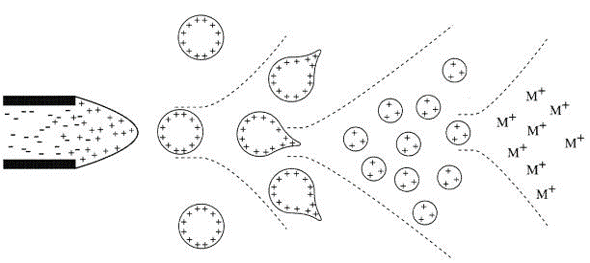
\includegraphics[width=3in]{Figures/Fig18.png}
            }
            \caption{Mechanism of Electrospray Ionization}
            \tiny{\url{https://en.wikipedia.org/wiki/Electrospray_ionization}}

        \end{figure}

        \subsubsection[\textbf{The Electrospray Ionization Mass Spectrometry Process}]{\textbf{The Electrospray Ionization Mass Spectrometry (ESI-MS) Process}} \hfill

        \begin{figure}[h]
            \centering
        
            \fbox{
                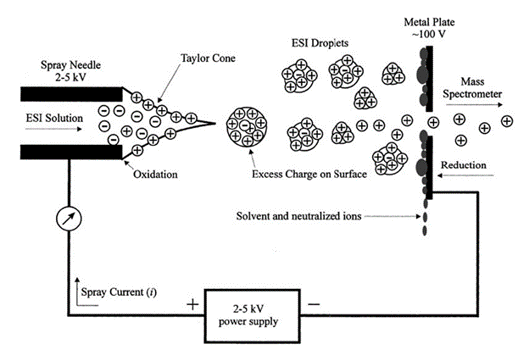
\includegraphics[width=3in]{Figures/Fig17.png}
            }
            \caption{Schematic Diagram of Electrospray Ionization Process\autocite{R6}}
        \end{figure}
 
            Since ion formation involves extensive solvent evaporation, the analyte needs to be dissolved in a volatile organic solvent such as methanol, sometimes in combination with acetic acid. High voltage (e.g. 2.5-6.0kV) is applied to the capillary needle resulting in the emission of aerosolized charged droplets of the sample. The charged droplets have the same charge as the capillary voltage that is applied.

                \begin{figure}[h]
                    \centering
                
                    \fbox{
                        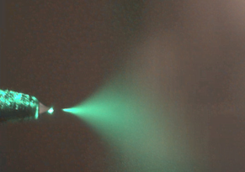
\includegraphics[width=3in]{Figures/Fig20.png}
                    }
                    \caption{Electrospray Plume Illuminated with A Green Laser}
                    \tiny{\url{http://rsl.eng.usf.edu/Pages/ResearchElectrosprayAmbient.html}}

                \end{figure}

            The charged droplets that are generated at the exit of the capillary pass down a pressure gradient. They are reduced in size by evaporation of the solvent with the aid of a continous flow of heated nitrogen drying gas; this leads to an increase of surface charge density and a decrease of the droplet radius. The strength of electric field within the charged droplet reaches a critical point at which it is kinetically and energetically possible for ions at the surface of the droplets to be ejected into the gaseous phase. The analysis of molecular mass and measurement of ion intensity begins after this phase.\autocite{R6}

            \FloatBarrier
        
%%%%%%%%%%%%%%%%%%%%%%%%%%%%%%%%%%%%%%%%%%%%%%%%%%%%%%%%%%%%%%%%%%%%%%%%%%%%%%%%
        \subsection{\textbf{ESI-MS Applications in Molecular Diagnostics}}
%%%%%%%%%%%%%%%%%%%%%%%%%%%%%%%%%%%%%%%%%%%%%%%%%%%%%%%%%%%%%%%%%%%%%%%%%%%%%%%%

%%%%%%%%%%%%%%%%%%%%%%%%%%%%%%%%%%%%%%%%%%%%%%%%%%%%%%%%%%%%%%%%%%%%%%%%%%%%%%%%
            \subsubsection[\textbf{Screeing for Inborn Errors of Metabolism}]{\textbf{Screening for Inborn Errors of Metabolism (ISM)}}\hfill

            \begin{figure}[h]
                \centering
            
                \fbox{
                    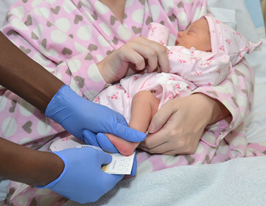
\includegraphics[width=3in]{Figures/Fig21.png}
                }
                \caption{Newborn Blood Spot Test}
                \tiny{\url{https://phescreening.blog.gov.uk/2016/08/18/new-format-to-uk-nsc-consultations-starts-with-5-newborn-blood-spot-conditions/}}
            \end{figure}

            ESI-MS provides early diagnosis and management of IEM disorders. Phenylketonuria (PKU) is an IEM that results in decreased metabolism of the amino acid phenylalanine. It can lead to permanent intellectual disability. In the past, PKU screening required a sufficient accumulation of phenylalanine in the infant's blood before successful positive diagnosis. Advances in MS technology have allowed PKU screening to be performed using day 1 blood spots. This is possible by utilizing ESI-MS to measure the phenylalanine to tyrosine concentration ratio in milliliter volume infant blood samples.

%%%%%%%%%%%%%%%%%%%%%%%%%%%%%%%%%%%%%%%%%%%%%%%%%%%%%%%%%%%%%%%%%%%%%%%%%%%%%%%%
           \subsubsection{\textbf{Identification and Quantification of Haemoglobin Variants}}\hfill

           ESI-MS has been revolutionary for identifying large bio-molecules and proteins within biochemical research. It has become the preferred technique for a rapid systematic approach to definitive characterization of Hb variants within diverse human populations.\autocite{R6}

%%%%%%%%%%%%%%%%%%%%%%%%%%%%%%%%%%%%%%%%%%%%%%%%%%%%%%%%%%%%%%%%%%%%%%%%%%%%%%%%
%%%%%%%%%%%%%%%%%%%%%%%%%%%%%%%%%%%%%%%%%%%%%%%%%%%%%%%%%%%%%%%%%%%%%%%%%%%%%%%%            
    \section{\textbf{Benefits and Limitations of MS in Molecular Diagnostics}}
%%%%%%%%%%%%%%%%%%%%%%%%%%%%%%%%%%%%%%%%%%%%%%%%%%%%%%%%%%%%%%%%%%%%%%%%%%%%%%%%
%%%%%%%%%%%%%%%%%%%%%%%%%%%%%%%%%%%%%%%%%%%%%%%%%%%%%%%%%%%%%%%%%%%%%%%%%%%%%%%%
        
    \begin{figure}[h]
        \centering
    
        \fbox{
            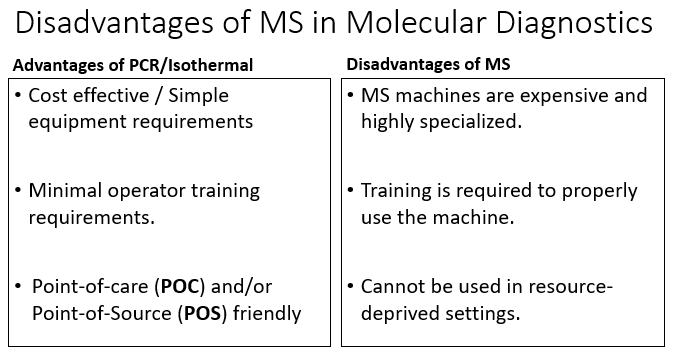
\includegraphics[width=3in]{Figures/Fig22.png}
        }
        \caption{Comparing MS with PCR and Isothermal for Molecular Diagnostic Applications}
    \end{figure}

%%%%%%%%%%%%%%%%%%%%%%%%%%%%%%%%%%%%%%%%%%%%%%%%%%%%%%%%%%%%%%%%%%%%%%%%%%%%%%%%
        \subsection[\textbf{Benefits}]{\textbf{Benefits\autocite{R1}}}
%%%%%%%%%%%%%%%%%%%%%%%%%%%%%%%%%%%%%%%%%%%%%%%%%%%%%%%%%%%%%%%%%%%%%%%%%%%%%%%%

The benefits of utilizing MS as a molecular diagnostics tool are largely based on the fact that it is a highly sensitive molecular detection system. For example, MS can detect sub-picomolar amounts of the analyte, precisely measure the size of a molecule of interest, and provide information on nucleotide composition and charge. 
Mass spectrometry is also great for analyzing contaminated samples such as feces or blood. The more commonly used PCR as molecular diagnostic technique fails with these fecal samples given they contain Taq DNA polymerase inhibitors which prevent use of traditional PCR techniques.\autocite{R11} MS, however, is able to easily identify bio-markers in contaminated samples due to the purely physical nature of its ionization process.

Speed is another advantage of using MS over conventional molecular diagnostic techniques, as target detection takes only milliseconds to seconds. This provides significant advantage, as techniques such as PCR or isothermal amplifications with subsequent gel electrophoresis can take hours. Even with the real time detections of amplified products, these processes cannot be completed in as short a time-frame as that provided using modern MS technology.

Lastly, the highly mechanized process of using MS can be coupled with automated sample preparation system to achieve high throughput diagnostics process. Since the sample loading and analysis process in MS is already heavily automated, it can be easily integrated into other high throughput technologies. Mass spectrometry systems are currently available which allow stacking of molecular arrays containing hundreds of samples for analysis without the necessitate of human intervention or monitoring.

%%%%%%%%%%%%%%%%%%%%%%%%%%%%%%%%%%%%%%%%%%%%%%%%%%%%%%%%%%%%%%%%%%%%%%%%%%%%%%%%        
        \subsection[\textbf{Limitations}]{\textbf{Limitations\autocite{R1}}}
%%%%%%%%%%%%%%%%%%%%%%%%%%%%%%%%%%%%%%%%%%%%%%%%%%%%%%%%%%%%%%%%%%%%%%%%%%%%%%%%

Although MS has been demonstrate to be an effective molecular diagnostics tool, it possesses several disadvantages when compared to conventionally applied molecular diagnostic methodologies such as PCR and isothermal DNA amplification techniques. 
While PCR and isothermal techniques are relatively cost effective, and do not require a overly complex machinery, MS systems are highly delicate and expensive instruments. The overall cost of purchasing, installing and operating the MS instruments are significantly higher than performing the same function using DNA amplification techniques.

Unlike the DNA amplification, which do not require extensive hands-on training for inexperienced personnel to operate, in-depth knowledge and training are required to properly operate MS instruments and analyze the output data. Furthermore, the MS technologies are currently not suitable for point-of-care or point-of-source diagnostic processes. With the advancement of DNA amplification technologies, there are now portable, USB battery charged PCR or isothermal devices that are available to be used in places where stable source of electricity is not available. The MS technologies have not achieved the portability and versatility of the DNA amplification technologies.\autocite{R11}

%%%%%%%%%%%%%%%%%%%%%%%%%%%%%%%%%%%%%%%%%%%%%%%%%%%%%%%%%%%%%%%%%%%%%%%%%%%%%%%%
%%%%%%%%%%%%%%%%%%%%%%%%%%%%%%%%%%%%%%%%%%%%%%%%%%%%%%%%%%%%%%%%%%%%%%%%%%%%%%%%
    \section{\textbf{Conclusion}}
%%%%%%%%%%%%%%%%%%%%%%%%%%%%%%%%%%%%%%%%%%%%%%%%%%%%%%%%%%%%%%%%%%%%%%%%%%%%%%%%
%%%%%%%%%%%%%%%%%%%%%%%%%%%%%%%%%%%%%%%%%%%%%%%%%%%%%%%%%%%%%%%%%%%%%%%%%%%%%%%%

Despite the disadvantages mentioned in the previous section, the fact that MS is a highly sensitive molecular detection technology remains true. Although the technology was initially regarded unsuitable for applications in the field of molecular diagnostics, the development of two soft ionization techniques, namely MALDI and ESI have enabled MS to become an effective molecular diagnostic tool. Because of these advancement in the ionization technologies, MS has been leveraged to achieve rapid and efficient diagnoses for a number of diseases including NEC and pancreatic cancer. 

Although the advancement in DNA amplification techniques has produced portable, cost-effective and easily used molecular diagnostic tools, MS has a major role in the field, especially with an increasing demand for a rapid, high throughput diagnostic methodologies. As the field of transcriptomics, proteomics and genomics continue to advance MS has an essential role to play in discovering and identifying bio-molecular targets for pharmaceutical intervention, molecular diagnostics, and other disciplines within molecular biology and medicine. Therefore pursuit training and familiarization of personnel with MS technology will be needed to ensure the rapid growth and deployment of new biotechnologies based on molecular identities or signatures. Through further application in molecular diagnostics, MS techniques will undoubtedly provide valuable insights into the cause, progress and treatment of human diseases.

%%%%%%%%%%%%%%%%%%%%%%%%%%%%%%%%%%%%%%%%%%%%%%%%%%%%%%%%%%%%%%%%%%%%%%%%%%%%%%%%%%%%%%%%%%%%%%%%%%%%%%%%%%%%%%%%%%%%%%%%%%%%%%%%%%%%%%%%%%%%%%%%%%%%%%%%%%%%%%%%
%%%%%%%%%%%%%%%%%%%%%%%%%%%%%%%%%%%%%%%%%%%%%%%%%%%%%%%%%%%%%%%%%%%%%%%%%%%%%%%%%%%%%%%%%%%%%%%%%%%%%%%%%%%%%%%%%%%%%%%%%%%%%%%%%%%%%%%%%%%%%%%%%%%%%%%%%%%%%%%%
%%%%%%%%%%%%%%%%%%%%%%%%%%%%%%%%%%%%%%%%%%%%%%%%%%%%%%%%%%%%%%%%%%%%%%%%%%%%%%%%%%%%%%%%%%%%%%%%%%%%%%%%%%%%%%%%%%%%%%%%%%%%%%%%%%%%%%%%%%%%%%%%%%%%%%%%%%%%%%%%

\addtolength{\textheight}{-12cm}  % This command serves to balance the column lengths
                                  % on the last page of the document manually. It shortens
                                  % the textheight of the last page by a suitable amount.
                                  % This command does not take effect until the next page
                                  % so it should come on the page before the last. Make
                                  % sure that you do not shorten the textheight too much.

%%%%%%%%%%%%%%%%%%%%%%%%%%%%%%%%%%%%%%%%%%%%%%%%%%%%%%%%%%%%%%%%%%%%%%%%%%%%%%%%

\printbibliography

%%%%%%%%%%%%%%%%%%%%%%%%%%%%%%%%%%%%%%%%%%%%%%%%%%%%%%%%%%%%%%%%%%%%%%%%%%%%%%%%

\end{document}
